\chapter{分解者与土壤}\label{ch:g6:decomposers-and-soil}

每年秋天，树林都会落下厚厚一层落叶——
每公顷可达数吨。可是每年春天再走进同一片树林，
并不会陷进越积越厚的落叶层：
落叶层年年都只是薄薄一层。是谁在吞食
森林中的枯死之物？本章深入\omterm{def:g6:decomposers-and-soil:soil}{土壤}，去认识这些
取食者——并最终闭合物质的循环。

\section{土壤是活的}

\begin{definition}[土壤]\label{def:g6:decomposers-and-soil:soil}
\emph{土壤}\index{土壤}是地球的“活\omterm{def:g1:the-five-senses:sense}{皮肤}”：一种由
\emph{矿物}颗粒（碾碎的岩石，从沙粒到黏土）、
\emph{有机}残体（处于各个分解阶段）、水、空气
以及数量庞大的\omterm{def:g6:exploring-our-environment:components}{生物}构成的混合物。其
表层颜色深暗，腐殖质最丰富，即
园丁们珍视的\emph{腐殖质}\index{腐殖质}层。
\end{definition}

\begin{example}[一把土的生物普查]\label{ex:g6:decomposers-and-soil:handful}
取一把林地\omterm{def:g6:decomposers-and-soil:soil}{土壤}，放在白色托盘上分拣：
矿物颗粒；根丝；半片落叶、叶片骨架；
以及黑色碎屑——正在分解的\omterm{def:g6:plants-are-producers:matter}{有机物}；还有
清点结果——一条蚯蚓、两只鼠妇、一只马陆、细小的
白色跳虫、细如丝线的\omterm{def:g6:decomposers-and-soil:decomposers}{真菌}菌丝团。托盘
上只能显示看得见的部分：一克\omterm{def:g6:decomposers-and-soil:soil}{土壤}
中藏着的肉眼看不见的\omterm{def:g6:exploring-our-environment:components}{生物}，多于
一座大城市的人口。
\end{example}

\begin{definition}[分解者]\label{def:g6:decomposers-and-soil:decomposers}
\emph{分解者}\index{分解者}是指
以\emph{死亡\omterm{def:g6:plants-are-producers:matter}{有机物}}为食的\omterm{def:g6:exploring-our-environment:components}{生物}——
如落叶、枯木、粪便和尸体：
\begin{itemize}
  \item 肉眼可见的“清扫队”：蚯蚓、鼠妇、马陆、
        跳虫、粪甲虫；
  \item \emph{真菌}\index{真菌}：霉菌和蘑菇，
        其取食体是由白色菌丝织成的毡状结构，
        遍布\omterm{def:g6:decomposers-and-soil:soil}{土壤}和枯木，而
        \cref{exo:g1:living-or-not:10}中的蘑菇只是它的\omterm{prop:g3:flowers-fruits-seeds:transform}{果实}；
  \item 还有负责收尾的、肉眼看不见的\omterm{def:g6:decomposers-and-soil:soil}{土壤}\omterm{def:g6:exploring-our-environment:components}{生物}——
        即最终的“拆解者”。
\end{itemize}
它们正是\cref{def:g5:food-webs:roles}所说的“幕后工作者”，
并承诺另列一章详述：本章便是。
\end{definition}

\section{分解：从有机物回到无机物}

\begin{proposition}[分解的作用]\label{prop:g6:decomposers-and-soil:decomposition}
\emph{分解}\index{分解}是\omterm{def:g6:decomposers-and-soil:decomposers}{分解者}的取食，
其结果恰与\omterm{def:g5:food-webs:roles}{生产者}的工作相反：
死亡的\emph{\omterm{def:g6:plants-are-producers:matter}{有机物}}被逐步拆解，
逐阶段、逐取食者地拆解，直至其物质
回到\emph{无机}世界——松散的\omterm{def:g6:decomposers-and-soil:soil}{腐殖质}，接着
溶于\omterm{def:g6:decomposers-and-soil:soil}{土壤}水中的\omterm{prop:g4:what-plants-need:needs}{无机盐}，以及
回到空气中的气体。秋天的落叶层，到春天时
恰好变为根所吸收的物质
（见\cref{prop:g4:what-plants-need:needs}）。
\end{proposition}
\admitted

\begin{example}[落叶的最后一年]\label{ex:g6:decomposers-and-soil:leaf}
跟踪一片橡树叶的去向。十一月：落地，完好无损。冬季：
变软，被\omterm{def:g6:decomposers-and-soil:decomposers}{真菌}菌丝侵蚀，
被跳虫和鼠妇啃成蕾丝状骨架。春季：
被蚯蚓拖入地下，吞食后，排出为
蚯蚓加工过的碎屑。夏季：其最后的碎片已成黑色
\omterm{def:g6:decomposers-and-soil:soil}{腐殖质}，其\omterm{prop:g4:what-plants-need:needs}{无机盐}随\omterm{def:g6:decomposers-and-soil:soil}{土壤}水移动，进入
根，或许正是这棵橡树自己的根。经四次取食，这片\omterm{def:g1:plants-around-us:parts}{叶子}
已成为它自己那棵树的食物。
\end{example}

\begin{omfigure}
\begin{tikzpicture}[scale=0.92]
  % cycle: producers -> consumers -> dead matter -> decomposers -> minerals -> producers
  \node[draw, thick, omMeth, fill=omMeth!8, rounded corners=4pt,
    font=\small, align=center] (prod) at (0,3.1)
    {生产者 \\ （植物）};
  \node[draw, thick, omExo, fill=omExo!8, rounded corners=4pt,
    font=\small, align=center] (cons) at (5.4,4.7)
    {消费者 \\ （动物）};
  \node[draw, thick, omProp, fill=omProp!8, rounded corners=4pt,
    font=\small, align=center] (dead) at (10.8,3.1)
    {遗体、\\ 粪便、落叶};
  \node[draw, thick, omThm, fill=omThm!8, rounded corners=4pt,
    font=\small, align=center] (dec) at (8.2,0.3)
    {分解者 \\ （土壤生物、真菌）};
  \node[draw, thick, omDef, fill=omDef!8, rounded corners=4pt,
    font=\small, align=center] (min) at (2.2,0.3)
    {矿物质：\\ 土壤水中的盐分};
  \draw[->, very thick, omDef] (prod.north east) -- (cons.west)
    node[midway, above=1pt, font=\footnotesize, sloped] {被取食};
  \draw[->, very thick, omDef] (cons.east) -- (dead.north west)
    node[midway, above=1pt, font=\footnotesize, sloped] {死亡、粪便};
  \draw[->, very thick, omDef] (prod.east) -- (dead.west)
    node[midway, below=1pt, font=\footnotesize] {落叶、枯木};
  \draw[->, very thick, omDef] (dead.south) -- (dec.north east)
    node[midway, right=2pt, font=\footnotesize] {取食};
  \draw[->, very thick, omDef] (dec.west) -- (min.east)
    node[midway, above=1pt, font=\footnotesize] {分解};
  \draw[->, very thick, omDef] (min.north) -- (prod.south east)
    node[midway, left=2pt, font=\footnotesize] {被根吸收};
\end{tikzpicture}

{\small 物质循环：由\omterm{def:g5:food-webs:roles}{生产者}制造，
经\omterm{def:g5:food-webs:roles}{消费者}传递，由\omterm{def:g6:decomposers-and-soil:decomposers}{分解者}归还，
再被\omterm{def:g5:food-webs:roles}{生产者}吸收。任何环节都不可或缺。}
\end{omfigure}

\begin{remark}[循环闭合]\label{rem:g6:decomposers-and-soil:circle}
\omterm{def:g6:decomposers-and-soil:decomposers}{分解者}就位后，本学年的物质故事
闭合成一个轮子：\omterm{def:g5:food-webs:roles}{生产者}由\omterm{def:g6:plants-are-producers:matter}{无机物}合成\omterm{def:g6:plants-are-producers:matter}{有机物}
（见\cref{ch:g6:plants-are-producers}）；\omterm{def:g5:food-webs:roles}{消费者}将其传递
（见\cref{ch:g6:matter-from-food}）；\omterm{def:g6:decomposers-and-soil:decomposers}{分解者}将其归还为
\omterm{def:g6:plants-are-producers:matter}{无机物}，再供\omterm{def:g5:food-webs:roles}{生产者}利用。物质不会被用尽
——它在循环流动。本页纸张中的原子
已经历过无数次成为叶、\omterm{def:g6:decomposers-and-soil:soil}{腐殖质}、根再成为叶的过程，
不可胜数。
\end{remark}

\section{与分解者打交道}

\begin{example}[堆肥，终于讲清楚]\label{ex:g6:decomposers-and-soil:compost}
\cref{ex:g2:caring-for-nature:compost}中的堆肥箱
现在可以理解为一件器具：一座堆满果皮的\omterm{def:g6:decomposers-and-soil:decomposers}{分解者}工坊
蚯蚓、潮虫和看不见的“工作队”
把厨房里的有机废物分解成深色的\omterm{def:g6:decomposers-and-soil:soil}{腐殖质}；园丁
将其铺撒，其中的\omterm{prop:g4:what-plants-need:needs}{无机盐}滋养苗床
（见\cref{rem:g4:what-plants-need:soil}）。堆肥甚至会发热——
这正是\omterm{def:g6:decomposers-and-soil:decomposers}{分解者}自身的燃烧
（见\cref{prop:g6:matter-from-food:losses}）使其
工坊升温。
\end{example}

\begin{proposition}[影响分解快慢的因素]\label{prop:g6:decomposers-and-soil:speed}
\omterm{def:g6:decomposers-and-soil:decomposers}{分解者}是对\omterm{def:g6:exploring-our-environment:conditions}{条件}有要求的\omterm{def:g6:exploring-our-environment:components}{生物}
（见\cref{prop:g6:exploring-our-environment:decide}）：它们在
\emph{温暖}、\emph{潮湿}且\emph{通气}时分解最快，
在冷、干燥或淹水缺氧时几乎停止。因此
秋季落叶在冬季缓慢分解，春季则很快被清除；
堆肥的做法也由此而来——保持湿润、
定期翻堆通气，切忌湿透封闭成团。
\end{proposition}
\admitted

\begin{method}[判断土壤健康状况]\label{met:g6:decomposers-and-soil:read}
用博物学家的方法判断\omterm{def:g6:decomposers-and-soil:soil}{土壤}：
\begin{enumerate}
  \item 挖出一掌深的土并观察：是深色松散的\omterm{def:g6:decomposers-and-soil:soil}{腐殖质}，还是
        灰白、毫无生气的尘土？
  \item 将一把土放在白色托盘上清点：蚯蚓、
        潮虫、弹尾虫。数量丰富的“工作队”说明循环
        正在运转；
  \item 检查表层：死亡\omterm{def:g6:plants-are-producers:matter}{有机物}是否随季节消失，
        还是堆积而未腐烂？
  \item 把“工作队”当作家畜来照料：为其提供食物（
        翻埋的残体、堆肥、覆盖物），保持湿润，避免
        毒物。
\end{enumerate}
\end{method}

\begin{example}[蚯蚓，园丁中的园丁]\label{ex:g6:decomposers-and-soil:worm}
蚯蚓身兼两职：\omterm{def:g6:decomposers-and-soil:decomposers}{分解者}——把树叶拖入地下、
取食腐烂物质；又是\emph{松土者}，
其洞穴使\omterm{def:g6:decomposers-and-soil:soil}{土壤}通气，其粪便将\omterm{def:g6:plants-are-producers:matter}{无机物}与\omterm{def:g6:plants-are-producers:matter}{有机物}
揉合在一起。一片草地下蚯蚓的体重
可以超过草地上奶牛的体重；旧时的
博物学家称蚯蚓为真正的农田“造田者”，
他们说得没错。
\end{example}

\begin{omfigure}
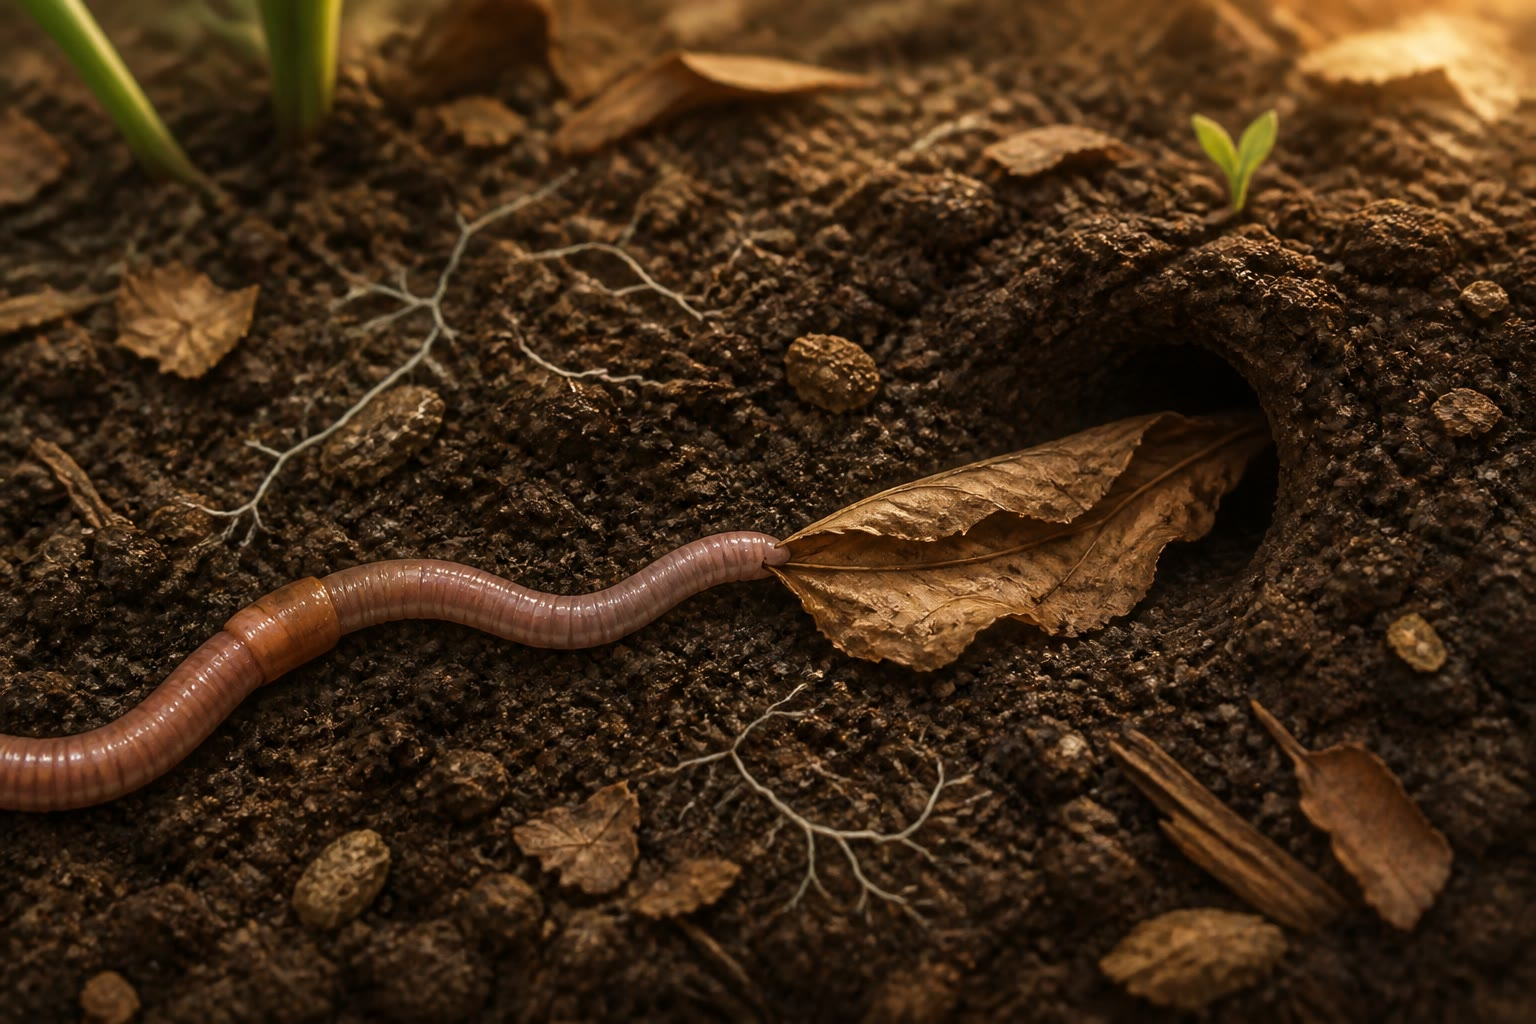
\includegraphics[width=0.6\linewidth]{images/book1/ai/g6-soil-earthworm.jpg}

{\small 农田的造田者正在工作：一片\omterm{def:g1:plants-around-us:parts}{叶子}正被拖往
地下，白色的\omterm{def:g6:decomposers-and-soil:decomposers}{真菌}菌丝已在
分解其他落叶。}
\end{omfigure}

\section{练习}

\begin{exercise}[$\star$]\label{exo:g6:decomposers-and-soil:1}
\omterm{def:g6:decomposers-and-soil:soil}{土壤}由什么构成？说出它的四种\omterm{def:g1:living-or-not:nonliving}{非生物}成分，
以及其中宝贵的深色土层。
\end{exercise}

\begin{exercise}[$\star$]\label{exo:g6:decomposers-and-soil:2}
\omterm{def:g6:decomposers-and-soil:decomposers}{分解者}以什么为食？列举四种肉眼可见的\omterm{def:g6:decomposers-and-soil:decomposers}{分解者}，
并说出一种取食部分是菌丝毡的\omterm{def:g6:decomposers-and-soil:decomposers}{分解者}。
\end{exercise}

\begin{exercise}[$\star$]\label{exo:g6:decomposers-and-soil:3}
说明分解作用会把\omterm{def:g6:plants-are-producers:matter}{有机物}变成什么——并
说明它逆转了哪一类\omterm{def:g6:exploring-our-environment:components}{生物}的工作。
\end{exercise}

\begin{exercise}[$\star$]\label{exo:g6:decomposers-and-soil:4}
用四季的顺序，讲述一片橡树叶最后一年的经历。
\end{exercise}

\begin{exercise}[$\star$]\label{exo:g6:decomposers-and-soil:5}
为什么森林里秋天落下的落叶层不会
年复一年地堆积起来？
\end{exercise}

\begin{exercise}[$\star$]\label{exo:g6:decomposers-and-soil:6}
\omterm{def:g6:decomposers-and-soil:decomposers}{分解者}在哪三种\omterm{def:g6:exploring-our-environment:conditions}{条件}下工作最快？
一年中何时分解变慢？为什么？
\end{exercise}

\begin{exercise}[$\star\star$]\label{exo:g6:decomposers-and-soil:7}
画出或描述物质循环，以及它的三类角色
——\omterm{def:g5:food-webs:roles}{生产者}、\omterm{def:g5:food-webs:roles}{消费者}和\omterm{def:g6:decomposers-and-soil:decomposers}{分解者}——并在
每两者之间各画一个箭头。
\end{exercise}

\begin{exercise}[$\star\star$]\label{exo:g6:decomposers-and-soil:8}
把堆肥箱解释为一座\omterm{def:g6:decomposers-and-soil:decomposers}{分解者}工坊：谁
在那里工作，加工什么，为花园产出什么——并
说明堆肥为什么会发热？
\end{exercise}

\begin{exercise}[$\star\star$]\label{exo:g6:decomposers-and-soil:9}
 说出蚯蚓的两项作用，以及旧时
博物学家为何称它为“农田的缔造者”。
\end{exercise}

\begin{exercise}[$\star\star$]\label{exo:g6:decomposers-and-soil:10}
对两种\omterm{def:g6:decomposers-and-soil:soil}{土壤}运用\cref{met:g6:decomposers-and-soil:read}：一块
铺有覆盖物的花圃，和一段裸露、被踩实的小路。
预测每一步的结果。
\end{exercise}

\begin{exercise}[$\star\star$]\label{exo:g6:decomposers-and-soil:11}
一只装有草屑的密封塑料袋，变成了发臭的
烂泥，而非堆肥。哪一项工作\omterm{def:g6:exploring-our-environment:conditions}{条件}被剥夺，
由\cref{prop:g6:decomposers-and-soil:speed}可知，
园丁又会做出怎样的改变？
\end{exercise}

\begin{exercise}[$\star\star\star$]\label{exo:g6:decomposers-and-soil:12}
“没有\omterm{def:g6:decomposers-and-soil:decomposers}{分解者}，\omterm{def:g5:food-webs:roles}{生产者}便会在
堆积如山的死亡之物中挨饿。”请论证
这句话的两部分，用物质循环说明——什么在堆积，以及
什么会耗尽？
\end{exercise}

\section{问题：落叶袋实验}

\begin{problem}[{周末问题——网袋、埋入的落叶，
以及一个冬季的土壤科学}]\label{pb:g6:decomposers-and-soil:1}
全班于十一月把落叶袋埋入学校的
树篱堤岸中：等重的新鲜橡树叶装入网袋，
待全年陆续挖出并重新称重。袋子分三类：
粗网袋（允许蚯蚓、潮虫等一切进入），
细网袋（挡住可见的\omterm{def:g1:animals-around-us:animal}{动物}群，只允许
看不见的\omterm{def:g6:exploring-our-environment:components}{生物}进入），以及密封塑料袋（挡住一切，
连空气也一并挡住）。

\medskip\noindent\textbf{第一部分——实验准备}
\begin{enumerate}
  \item 为什么所有袋子都必须装\emph{同样}重量的
        \emph{同种}落叶，并于\emph{同一天}埋下，
        埋在\emph{同一}堤岸中？请说出所用的方法。
  \item 细网袋能提出怎样的问题，
        是粗网袋单独无法提出的？
  \item 有一组同学想增加第四个袋子：粗网袋，
        但埋在操场上干燥的砾石中。它会
        提出什么问题，依据
        \cref{prop:g6:decomposers-and-soil:speed}？
  \item 挖掘之前先作预测：将树篱堤岸中的三个袋子
        按到六月为止将损失的落叶重量排序，
        （从多到少）。
\end{enumerate}

\medskip\noindent\textbf{第二部分——实验结果}
\begin{enumerate}[resume]
  \item 六月的称重：粗网袋——重量减少最多，
        叶片只剩骨架和碎屑；细网袋——
        明显变轻，叶片变软、变黑，但速度较慢；密封塑料袋——
        重量几乎不变，内容物成了发酸的烂泥。
        请解释
        每个袋子的情况。
  \item 全班在粗网袋中发现了潮虫、一条
        蚯蚓、弹尾虫和白色的\omterm{def:g6:decomposers-and-soil:decomposers}{真菌}菌丝。请为
        每一类\omterm{def:g6:exploring-our-environment:components}{生物}指明它们在落叶分解中的作用
        （\cref{ex:g6:decomposers-and-soil:leaf}为
        范例）。
  \item 细网袋确实减轻了重量，尽管
        所有可见\omterm{def:g1:animals-around-us:animal}{动物}都已被挡在外面，这说明
        看不见的\omterm{def:g6:decomposers-and-soil:soil}{土壤}\omterm{def:g6:exploring-our-environment:components}{生物}具有什么作用？
  \item 砾石操场中的袋子（第 3 题中的那只）减少的重量
        远少于它在树篱堤岸中的孪生袋子。哪些工作\omterm{def:g6:exploring-our-environment:conditions}{条件}
        被砾石所剥夺？
\end{enumerate}

\medskip\noindent\textbf{第三部分——更深一层的启示}
\begin{enumerate}[resume]
  \item 粗网袋损失的重量\emph{去了}哪里？
        请借助
        \cref{prop:g6:decomposers-and-soil:decomposition}
        ——至少给出两个去向。
  \item 树篱中的荨麻在春季
        恰好在全班埋放网袋的那段堤岸边长得最为青绿。这
        是否只是巧合？请从物质循环出发论证。
  \item 利用密封袋解释：为什么被填埋的有机废物，
        以塑料气密包裹后，
        会存留数十年，而同样的废物
        只需几个月便能变成堆肥。
  \item 用两句话作结：这个冬季
        证明了谁在清理森林的地被，
        这种清理又滋养了什么？
\end{enumerate}
\end{problem}
